\subsection{Диаграмма вариантов использования}

На рисунке представлена диаграмма вариантов использования, демонстрирующая взаимодействие пользователей с системой. Каждый пользователь (актёр) обладает определённым набором действий, доступных в рамках его роли:

\begin{itemize}
    \item \textbf{Преподаватель} — создание и управление группами и заданиями, взаимодействие со студентами в чатах, а также анализ кода лабораторных работ с использованием AI;
    \item \textbf{Студент} — участие в групповых и личных чатах, выполнение заданий и просмотр результатов;
    \item \textbf{Администратор} — управление институтами, кафедрами, группами, студентами и преподавателями, а также создание приглашений в систему.
\end{itemize}

\begin{figure}[H]
\centering
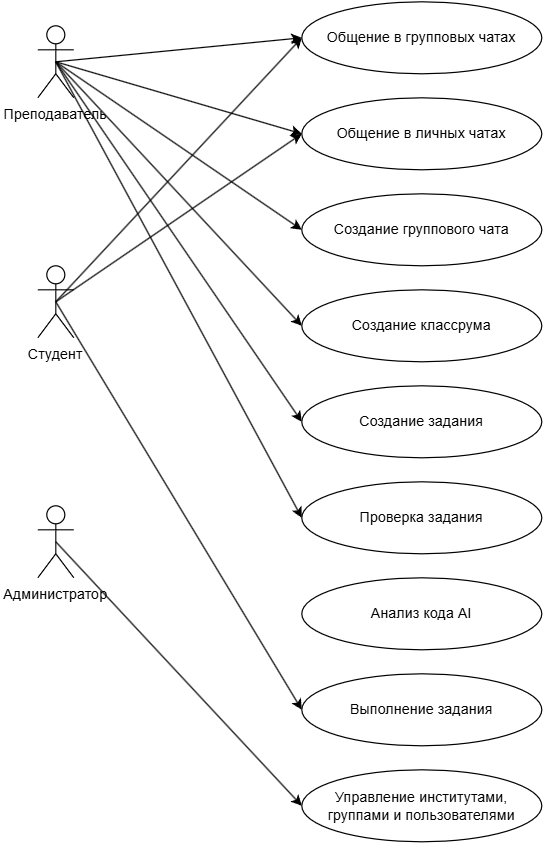
\includegraphics[width=0.5\linewidth]{static/useCaseDiagramm}
\caption{Диаграмма вариантов использования системы для различных ролей пользователей.}
\label{fig:usecasediagramm}
\end{figure}